\documentclass[12pt, a4paper]{article}
\usepackage[utf8]{inputenc}
\usepackage[margin=20mm]{geometry}

\usepackage{lmodern}

\usepackage{hyperref}
\hypersetup{
    colorlinks=true, % make the links colored
    linkcolor=black, % color TOC links in blue
    linktoc=all % 'all' will create links for everything in the TOC
}

\usepackage[inter-unit-product =\cdot]{siunitx}

\usepackage{amsmath}
\usepackage{amsfonts}

\usepackage[usenames, dvipsnames]{xcolor}

\usepackage{tcolorbox}

\usepackage{pgfplots}
\pgfplotsset{compat=1.9}

\usepackage{tikz}
\usetikzlibrary{arrows}
\tikzset{vecteur/.style={->, very thick, >=stealth}}
\tikzset{point/.style={color=darkgray}}
\tikzset{festat/.style={color=Green}}
\tikzset{unitaire/.style={color=violet}}
\tikzset{cestat/.style={color=blue}}

\usepackage[tikz]{bclogo}


\newcommand{\myparagraph}[1]{\paragraph{#1}\mbox{}\\}
\newcommand*\mean[1]{\overline{#1}}

\usepackage{scalerel,stackengine}
\stackMath

\newcommand\reallywidehat[1]{%
\savestack{\tmpbox}{\stretchto{%
  \scaleto{%
    \scalerel*[\widthof{\ensuremath{#1}}]{\kern-.6pt\bigwedge\kern-.6pt}%
    {\rule[-\textheight/2]{1ex}{\textheight}}%WIDTH-LIMITED BIG WEDGE
  }{\textheight}% 
}{0.5ex}}%
\stackon[1pt]{#1}{\tmpbox}%
}







\title{\textbf{Transformations de Fourier}}
\author{\textit{Robin SHAMSNEJAD, cours de François BLANCHET (Polytech E2I)}}
\date{}

\begin{document}

\maketitle

\tableofcontents
\clearpage

\section{Outils}

\subsection{Fonctions remarquables}

\subsubsection{Fonction indicatrice}

\begin{tcolorbox}
	On appelle << indicatrice de $[a, b]$ >> la fonction définie par :
	\begin{equation*}
		\forall (a, b, x) \in \mathbb{R}^3, X_{[a, b]}(x) =
		\begin{cases}
			1 ~ \text{si} ~ x \in [a, b] \\
			0 ~ \text{sinon}
		\end{cases}
	\end{equation*}
\end{tcolorbox}

Par exemple, voici la représentation de la fonction $X_{[1, 3]}$ :

\begin{center}
	\begin{tikzpicture}
		\begin{axis}[axis lines=middle, height=5cm, width=15cm]
			\addplot[domain=-1:5, samples=100, color=red]
				coordinates {(-1,0) (1,0)};
			\addplot[domain=-1:5, samples=100, color=red]
				coordinates {(1,1) (3,1)};
			\addplot[domain=-1:5, samples=100, color=red]
				coordinates {(3,0) (5,0)};
			\addlegendentry{$X_{[1, 3]}(x)$}
		\end{axis}
	\end{tikzpicture}
\end{center}

\subsubsection{Fonction porte}

La fonction porte est un cas particulier de la fonction indicatrice, et est une première fonction de référence que l'on utilisera dans les transformations de Fourier :

\begin{tcolorbox}
	La fonction << porte >> est définie par :
	\begin{equation*}
		\forall x \in \mathbb{R}, \Pi(x) = X_{[-\frac{1}{2}, \frac{1}{2}]}(x)
	\end{equation*}
\end{tcolorbox}

\begin{center}
	\begin{tikzpicture}
		\begin{axis}[axis lines=middle, height=5cm, width=15cm]
			\addplot[domain=-1:1, samples=100, color=red]
				coordinates {(-2,-0) (-0.5,0)};
			\addplot[domain=-1:1, samples=100, color=red]
				coordinates {(-0.5,1) (0.5,1)};
			\addplot[domain=-1:1, samples=100, color=red]
				coordinates {(0.5,0) (2,0)};
			\addlegendentry{$\Pi(x)$}
		\end{axis}
	\end{tikzpicture}
\end{center}


\clearpage


\subsubsection{Fonction triangle}

La fonction triangle est une deuxième fonction de référence pour les transformations de Fourier :

\begin{tcolorbox}
	La fonction << triangle >> est définie par :
	\begin{equation*}
		\forall x \in \mathbb{R}, \Lambda(x) =
		\begin{cases}
			x + 1 ~ \text{si} ~ x \in [-1, 0] \\
			-x + 1 ~ \text{si} ~ x \in [0, 1] \\
			0 ~ \text{sinon}
		\end{cases}
	\end{equation*}
\end{tcolorbox}

\begin{center}
	\begin{tikzpicture}
		\begin{axis}[axis lines=middle, height=5cm, width=15cm]
			\addplot[domain=-1:1, samples=100, color=red] 
				coordinates {(-2,-0) (-1,0) (0,1) (1,0) (2,0)};
			\addlegendentry{$\Lambda(x)$}
		\end{axis}
	\end{tikzpicture}
\end{center}

\subsubsection{Fonction signe}

La fonction << signe >> n'est pas une fonction de référence, mais est utile pour certains calculs.

\begin{tcolorbox}
	La fonction << signe >> est définie par :
	\begin{equation*}
		\forall x \in \mathbb{R}, signe(x) = 
		\begin{cases}
			-1 \text{ si } x < 0 \\
			0 \text{ si } x = 0 \\
			1 \text{ si } x > 0
		\end{cases}
	\end{equation*}
	Elle peut également s'écrire de la façon suivante :
	\begin{equation*}
		\forall x \in \mathbb{R}, signe(x) = 
		\begin{cases}
			0 \text{ si } x = 0 \\
			\displaystyle \frac{x}{|x|}, \forall x \in \mathbb{R}^*
		\end{cases}
	\end{equation*}
\end{tcolorbox}

\begin{center}
	\begin{tikzpicture}
		\begin{axis}[axis lines=middle, height=5cm, width=15cm]
			\addplot[domain=-10:10, samples=100, color=red]
				coordinates {(-10,-1) (0,-1)};
			\addplot[domain=-10:10, samples=100, color=red]
				coordinates {(0,1) (10,1)};
			\addlegendentry{$signe(x)$}
		\end{axis}
	\end{tikzpicture}
\end{center}


\clearpage


\subsubsection{Fonction sinus cardinal}

Le sinus cardinal est une troisième fonction de référence pour les transformations de Fourier :

\begin{tcolorbox}
	La fonction << sinus cardinal >> est définie par :
	\begin{equation*}
		\forall x \in \mathbb{R}, sinc(x) = \frac{sin(\pi x)}{\pi x}
	\end{equation*}
\end{tcolorbox}

\begin{center}
	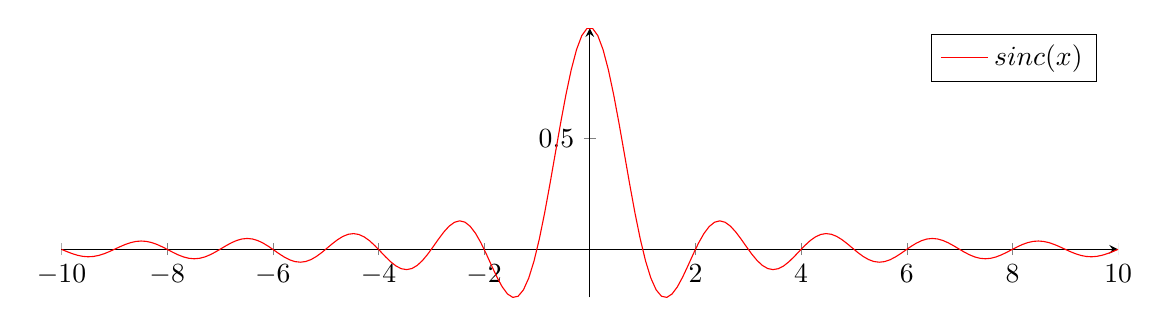
\begin{tikzpicture}
		\begin{axis}[axis lines=middle, height=5cm, width=15cm]
			\addplot[domain=-10:10, samples=200, color=red] {sin(pi*deg(x))/(pi*x)};
			\addlegendentry{$sinc(x)$}
		\end{axis}
	\end{tikzpicture}
\end{center}

\subsection{Contraction et translation de fonctions}

Les opérations de << contraction >> et de << translation >> de fonctions, au sens graphique, est un outil qui permettra de ramener certaines fonctions à des fonctions de référence << modifiées >> pour calculer facilement leur transformation de Fourier.

\subsubsection{Translation}

Pour translater une fonction de $a$ vers la droite, il faut \textbf{retirer $a$ de la variable} :

\begin{tcolorbox}
	La translation d'une fonction $f:\mathbb{R} \to \mathbb{R}$ d'un facteur $a$ dans le sens de l'axe des abcisses est définie par :
	\begin{equation*}
		\forall (x, a) \in \mathbb{R}^2, T_{a}f(x) = f(x - a)
	\end{equation*}
	
	ATTENTION : le terme $x - a$ doit \textbf{\emph{remplacer}} $x$ ! Il ne faut surtout par retirer $a$ à toute la fonction.
\end{tcolorbox}

\begin{center}
	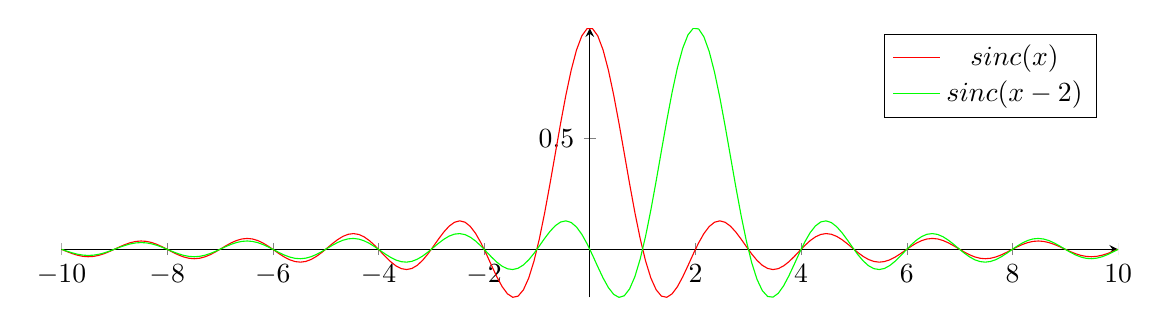
\begin{tikzpicture}
		\begin{axis}[axis lines=middle, height=5cm, width=15cm]
			\addplot[domain=-10:10, samples=200, color=red] {sin(pi*deg(x))/(pi*x)};
			\addlegendentry{$sinc(x)$}
			\addplot[domain=-10:10, samples=200, color=green] {sin(pi*deg(x-2))/(pi*(x-2))};
			\addlegendentry{$sinc(x-2)$}
		\end{axis}
	\end{tikzpicture}
\end{center}


\clearpage


Pour décaler (on ne parle pas de << translater >> ici) une fonction de $a$ vers le haut, il faut \textbf{ajouter $a$ à toute la fonction} :

\begin{center}
	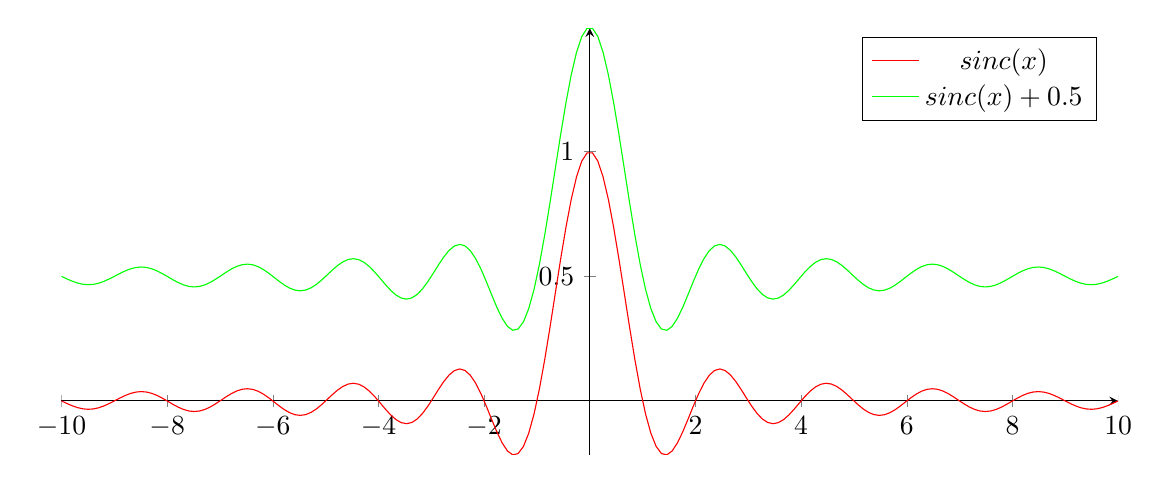
\begin{tikzpicture}
		\begin{axis}[axis lines=middle, height=7cm, width=15cm]
			\addplot[domain=-10:10, samples=200, color=red] {sin(pi*deg(x))/(pi*x)};
			\addlegendentry{$sinc(x)$}
			\addplot[domain=-10:10, samples=200, color=green] {0.5 + sin(pi*deg(x))/(pi*(x))};
			\addlegendentry{$sinc(x) + 0.5$}
		\end{axis}
	\end{tikzpicture}
\end{center}

\subsubsection{Contraction}

Pour contracter une fonction d'un facteur $a$ autour de l'axe des des ordonnées, il faut \textbf{multiplier la variable par $a$} :

\begin{tcolorbox}
	La contraction d'une fonction $f:\mathbb{R} \to \mathbb{R}$ d'un facteur $a$ autour de l'axe des des ordonnées est définie par :
	\begin{equation*}
		\forall (x, a) \in \mathbb{R}^2, C_{a}f(x) = f(a\cdot x)
	\end{equation*}
	
	ATTENTION : le terme $a \cdot x$ doit \textbf{\emph{remplacer}} $x$ ! Il ne faut surtout par multiplier toute la fonction par $a$.
\end{tcolorbox}

\begin{center}
	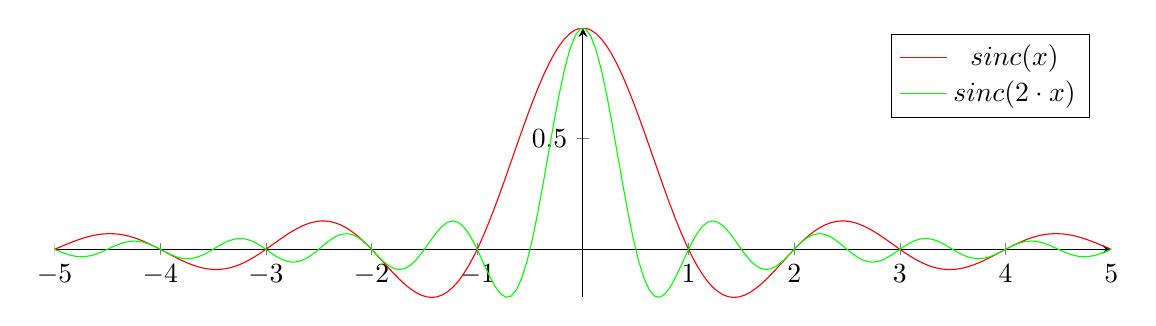
\begin{tikzpicture}
		\begin{axis}[axis lines=middle, height=5cm, width=15cm]
			\addplot[domain=-5:5, samples=200, color=red] {sin(pi*deg(x))/(pi*x)};
			\addlegendentry{$sinc(x)$}
			\addplot[domain=-5:5, samples=200, color=green] {sin(pi*deg(2*x))/(pi*(2*x))};
			\addlegendentry{$sinc(2 \cdot x)$}
		\end{axis}
	\end{tikzpicture}
\end{center}

Pour comprimer (on ne parle pas de << contracter >> ici) une fonction d'un facteur $a$ autour de l'axe des abcisses, il faut \textbf{diviser toute la fonction par $a$} :

\begin{center}
	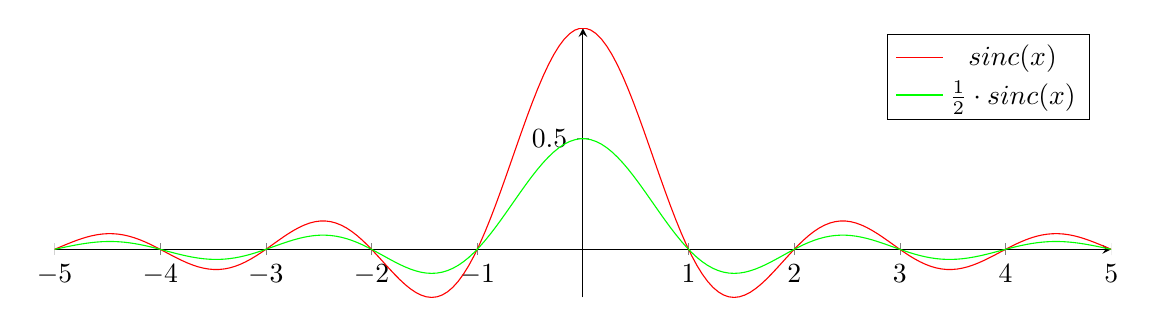
\begin{tikzpicture}
		\begin{axis}[axis lines=middle, height=5cm, width=15cm]
			\addplot[domain=-5:5, samples=200, color=red] {sin(pi*deg(x))/(pi*x)};
			\addlegendentry{$sinc(x)$}
			\addplot[domain=-5:5, samples=200, color=green] {sin(pi*deg(x))/(pi*(2*x))};
			\addlegendentry{$\frac{1}{2} \cdot sinc(x)$}
		\end{axis}
	\end{tikzpicture}
\end{center}


\clearpage


\myparagraph{Remarque}

Contracter d'un facteur $\displaystyle \frac{1}{a}$ revient à \textbf{dilater d'un facteur $a$} (et il en va de même pour la compression) :

\begin{center}
	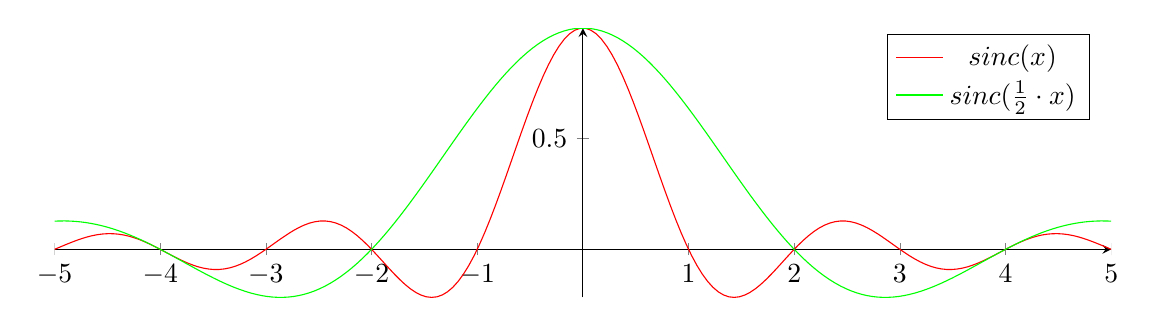
\begin{tikzpicture}
		\begin{axis}[axis lines=middle, height=5cm, width=15cm]
			\addplot[domain=-5:5, samples=200, color=red] {sin(pi*deg(x))/(pi*x)};
			\addlegendentry{$sinc(x)$}
			\addplot[domain=-5:5, samples=200, color=green] {sin(pi*deg(x/2))/(pi*(x/2))};
			\addlegendentry{$sinc(\frac{1}{2} \cdot x)$}
		\end{axis}
	\end{tikzpicture}
\end{center}

\begin{center}
	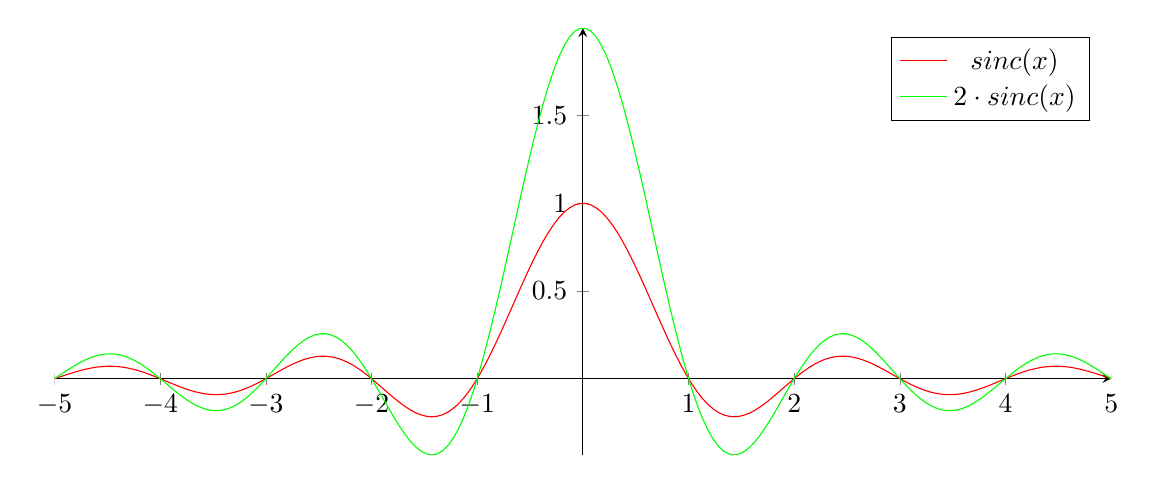
\begin{tikzpicture}
		\begin{axis}[axis lines=middle, height=7cm, width=15cm]
			\addplot[domain=-5:5, samples=200, color=red] {sin(pi*deg(x))/(pi*x)};
			\addlegendentry{$sinc(x)$}
			\addplot[domain=-5:5, samples=200, color=green] {2*sin(pi*deg(x))/(pi*(x))};
			\addlegendentry{$2 \cdot sinc(x)$}
		\end{axis}
	\end{tikzpicture}
\end{center}

\subsubsection{Miroir}

Un cas particulier de contraction est la contraction par $-1$ : il s'agit en fait de prendre la symétrie selon l'axe des ordonnées de la fonction : c'est comme si on regardait son reflet dans un miroir.

Donc si on contracte une fonction d'un facteur $-a$, elle est contractée de $a$, puis pivotée.

\begin{tcolorbox}
	Le cas particulier de la contraction d'une fonction par $-1$, qui donne sa symétrie selon l'axe des ordonnées, est noté $f_{\sigma}$ :
	\begin{equation*}
		f_{\sigma}(t) = C_{-1}f(t) = f(-t)
	\end{equation*}
\end{tcolorbox}


\section{Transformées de Fourier}

La transformation de Fourier est une sorte << d'extension >>, pour les fonctions non périodiques, du développement en série de Fourier des fonctions périodiques. La transformation de Fourier associe à une fonction intégrable définie sur $\mathbb{R}$ et à valeurs réelles ou complexes, une autre fonction sur $\mathbb{R}$ appelée \textbf{transformée de Fourier}. Cette nouvelle fonction a une variable indépendante de la fonction d'origine. Si la fonction d'origine a pour variable le temps (= le \textbf{signal}), la variable de sa transformée est la fréquence ou la pulsation (= le \textbf{spectre}).

\subsection{Définition}

\begin{tcolorbox}
	La fonction résultante de la la transformation de Fourier de la fonction $f:\mathbb{R} \to \mathbb{C}$ est appelée \textbf{transformée de Fourier} et est définie par :
	\begin{equation*}
		\mathcal{F}f(\xi) = \reallywidehat{f}(\xi) = \int_{\mathbb{R}}\left( f(t)\cdot e^{\displaystyle-i2\pi\xi t} \right)dt
	\end{equation*}
	
	Si cette transformée existe, alors on note $\displaystyle f \in L^{1}$, et, dans le cadre de ce cours, on considère que cela implique que $\displaystyle\int_{\mathbb{R}}|f(t)|dt$ converge.
\end{tcolorbox}

\subsection{Premières transformées remarquables}

\subsubsection{Fonction indicatrice}

Soient $a$ et $b$ deux réels :

\begin{equation*}
	\begin{aligned}
		\reallywidehat{X_{[a,b]}}(\xi) & = \int_{-\infty}^{+\infty} \left( X_{[a,b]}(t) \cdot e^{\displaystyle-i2\pi\xi t} \right) dt \\
		{} & = \int_{a}^{b} \left( X_{[a,b]}(t) \cdot e^{\displaystyle-i2\pi\xi t} \right) dt \\
		{} & = \int_{a}^{b} \left( e^{\displaystyle-i2\pi\xi t} \right) dt \\
		(\forall \xi \neq 0) & = \frac{-1}{i2\pi\xi} \left[ e^{\displaystyle-i2\pi\xi t} \right]_a^b \\
		{} & = \frac{e^{\displaystyle-i2\pi\xi b} - e^{\displaystyle-i2\pi\xi a}}{-i2\pi\xi} \\
		{} & = e^{\displaystyle-i\pi\xi (a+b)} \cdot \frac{e^{\displaystyle i\pi\xi (a-b)} - e^{\displaystyle-i\pi\xi (a-b)}}{-i2\pi\xi} \\
		{} & = e^{\displaystyle-i\pi\xi (a+b)} \cdot \frac{sin\left((b-a)\pi\xi\right)}{\pi\xi}
	\end{aligned}
\end{equation*}

\subsubsection{Fonction porte}

On réutilise la transformée de l'indicatrice calculée précédemment :

\begin{equation*}
	\begin{aligned}
		\reallywidehat{\Pi}(\xi) & = \reallywidehat{X_{[-\frac{1}{2},\frac{1}{2}]}}(\xi) \\
		{} & = \frac{sin(\pi\xi)}{\pi\xi} \\
		{} & = sinc(\xi)
	\end{aligned}
\end{equation*}

\begin{tcolorbox}
	La transformée de Fourier de la fonction porte est le sinus cardinal :
	\begin{equation*}
		\reallywidehat{\Pi} = sinc
	\end{equation*}
\end{tcolorbox}

\subsection{Propriétés des transformées de Fourier}

\subsubsection{Linéarité}

\begin{tcolorbox}
	Si on a deux fonctions $f$ et $g$ de classe $L^1$ :
	\begin{equation*}
		\forall (a, b) \in \mathbb{C}^2, ~ \reallywidehat{a\cdot f + b\cdot g} = a\cdot\reallywidehat{f} + b\cdot\reallywidehat{g}
	\end{equation*}
\end{tcolorbox}

\subsubsection{Transformée prise en 0}

\begin{tcolorbox}
	Soit $f \in L^1$ :
	\begin{equation*}
		\reallywidehat{f}(0) = \int_{\mathbb{R}}\left( f(t)\cdot e^{0} \right)dt = \int_{\mathbb{R}}f(t)dt
	\end{equation*}
	
	Le nombre $\reallywidehat{f}(0)$ représente donc l'aire totale sous la courbe de $f$.
\end{tcolorbox}

\subsubsection{Continuité et limite en l'infini (théorème de Riemann-Lebesgue)}

\begin{tcolorbox}
	Si $f$ admet une transformée de Fourier, alors $\reallywidehat{f}$ est continue et tend vers 0 en $+\infty$ et $-\infty$ :
	\begin{equation*}
		\forall f \in L^1,
		\begin{cases}
			\reallywidehat{f} \in C^0 \\
			\displaystyle \lim_{\xi \to +\infty} \reallywidehat{f}(\xi) = \lim_{\xi \to -\infty} \reallywidehat{f}(\xi) = 0
		\end{cases}
	\end{equation*}
\end{tcolorbox}

\subsubsection{Formule d'échange (conséquence du théorème de Fubini)}

\begin{tcolorbox}
	Soient $f$ et $g$ deux fonctions de classe $L^1$, alors :
	\begin{equation*}
		\begin{cases}
			\reallywidehat{f}\cdot g \in L^1 \\
			f \cdot \reallywidehat{g} \in L^1 \\
			\displaystyle \int_{\mathbb{R}}\reallywidehat{f}\cdot g = \int_{\mathbb{R}}f\cdot\reallywidehat{g}
		\end{cases}
	\end{equation*}
	$\rightarrow$ On peut << échanger les chapeaux >> au sein de l'intégrale.
\end{tcolorbox}

\subsubsection{Parité}

Soit $f \in L^1$ :

\begin{equation*}
	\begin{aligned}
		\reallywidehat{f}(\xi) & = \int_{-\infty}^{+\infty}\left( f(t)\cdot e^{\displaystyle-i2\pi\xi t} \right)dt \\
		{} & = \int_{-\infty}^{+\infty}\left[ f(t)\cdot(cos(-2\pi\xi t) + i\cdot sin(-2\pi\xi t)) \right]dt \\
		{} & = \int_{-\infty}^{+\infty}\left[ f(t)\cdot(cos(2\pi\xi t) - i\cdot sin(2\pi\xi t)) \right]dt \\
		{} & = \underbrace{\int_{-\infty}^{+\infty}\left[ f(t)\cdot cos(2\pi\xi t)\right]dt}_{\text{$= 0$ si $f$ est impaire}} - i\cdot \underbrace{\int_{-\infty}^{+\infty}\left[ f(t)\cdot sin(2\pi\xi t) \right]dt}_{\text{$= 0$ si $f$ est paire}}
	\end{aligned}
\end{equation*}

\begin{tcolorbox}
	Soit $f \in L^1$
	\begin{itemize}
		\item Si $f$ est paire :
			\begin{equation*}
				\reallywidehat{f}(\xi) = \int_{-\infty}^{+\infty}\left[ f(t)\cdot cos(2\pi\xi t)\right]dt = 2\cdot \int_{0}^{+\infty}\left[ f(t)\cdot cos(2\pi\xi t)\right]dt
			\end{equation*}
		\item Si $f$ est impaire :
			\begin{equation*}
				\reallywidehat{f}(\xi) = -i\cdot \int_{-\infty}^{+\infty}\left[ f(t)\cdot sin(2\pi\xi t)\right]dt = -2i\cdot \int_{0}^{+\infty}\left[ f(t)\cdot sin(2\pi\xi t)\right]dt
			\end{equation*}
	\end{itemize}
\end{tcolorbox}

\subsubsection{Transformée et contraction/translation}

\myparagraph{Translations}

\begin{tcolorbox}
	Soient $f \in L^1$ et $a \in \mathbb{R}$
	\begin{itemize}
		\item La transformée de $f$ translatée de $a$ vaut :
			\begin{equation*}
				\reallywidehat{T_{a}f}(\xi) = e^{\displaystyle -i2\pi a\xi}\cdot\reallywidehat{f}(\xi)
			\end{equation*}
		\item La translatée de $a$ de la transformée de $f$ vaut :
			\begin{equation*}
				T_{a}\reallywidehat{f} = \reallywidehat{\underbrace{e^{\displaystyle i2\pi a t}}_{\text{\parbox{2cm}{ATTENTION : le signe moins a sauté}}}\cdot f(t)}
			\end{equation*}
	\end{itemize}
\end{tcolorbox}

\myparagraph{Contractions}

Soient $f \in L^1$ et $a \in \mathbb{R}^*$ :

\begin{equation*}
	\begin{aligned}
		\reallywidehat{C_{a}f}(\xi) & = \int_{\mathbb{R}}\left[ C_{a}f(t) \cdot e^{\displaystyle -i2\pi\xi t} \right]dt \\
		{} & = \int_{-\infty}^{+\infty}\left[ f(a\cdot t) \cdot e^{\displaystyle -i2\pi\xi t} \right]dt
	\end{aligned}
\end{equation*}

Si on fait le changement de variable $x = a\cdot t$, on a $dx = a \cdot dt$, et les bornes de l'intégrales sont inversées dans le cas où $a$ est négatif. Ainsi :

\begin{equation*}
	\begin{aligned}
		\reallywidehat{C_{a}f}(\xi) & = signe(a) \cdot \int_{-\infty}^{+\infty}\left[ f(x) \cdot e^{\displaystyle -i2\pi\xi \frac{x}{a}} \right]\frac{dx}{a} \\
		{} & = \frac{signe(a)}{a} \cdot \int_{-\infty}^{+\infty}\left[ f(x) \cdot e^{\displaystyle -i2\pi\xi \frac{x}{a}} \right]dx
	\end{aligned}
\end{equation*}


\clearpage


Or, $\displaystyle \frac{signe(a)}{a} = \frac{1}{a}\cdot \frac{a}{|a|} = \frac{1}{|a|}$

Ainsi :

\begin{equation*}
	\begin{aligned}
		\reallywidehat{C_{a}f}(\xi) & = \frac{1}{|a|} \cdot \int_{-\infty}^{+\infty}\left[ f(x) \cdot e^{\displaystyle -i2\pi\xi \frac{x}{a}} \right]dx \\
		{} & = \frac{1}{|a|} \cdot \int_{-\infty}^{+\infty}\left[ f(x) \cdot e^{\displaystyle -i2\pi\frac{\xi}{a}x} \right]dx \\
		{} & = \frac{1}{|a|} \cdot \reallywidehat{f}\left(\frac{1}{a}\cdot\xi\right) \\
		{} & = \frac{1}{|a|} \cdot C_{\frac{1}{a}}\reallywidehat{f}(\xi)
	\end{aligned}
\end{equation*}

\begin{tcolorbox}
	Soient $f \in L^1$ et $a \in \mathbb{R}^*$.
	
	La transformée de $f$ contractée de $a$ vaut :
	
	\begin{equation*}
		\reallywidehat{C_{a}f} = \frac{1}{|a|} \cdot C_{\frac{1}{a}}\reallywidehat{f}
	\end{equation*}
\end{tcolorbox}

Cela signifie que si on contracte une fonction, sa transformée se retrouve dilatée. Cela semble intuitif quand on considère l'interprétation physique : une forme d'onde contractée correspond à un signal de plus haute fréquence, et donc le spectre se retrouve dilaté.

\myparagraph{Combinaison de contraction et translation}

Soient $f \in L^1$ et $(a,b) \in \mathbb{R}^2$.

\begin{equation*}
		\begin{aligned}
			\reallywidehat{f(a\cdot t + b)}(\xi) & = \reallywidehat{f(a\cdot [t + \frac{b}{a}])}(\xi) \\
			{} & = \reallywidehat{T_{-\frac{b}{a}}C_{a}f}(\xi) \\
			{} & = e^{\displaystyle i2\pi\frac{b}{a}\xi} \cdot \reallywidehat{C_{a}f}(\xi) \\
			{} & = e^{\displaystyle i2\pi\frac{b}{a}\xi} \cdot \frac{1}{|a|} \cdot \reallywidehat{f}\left(\frac{1}{a}\cdot\xi\right)
		\end{aligned}
	\end{equation*}

\begin{tcolorbox}
	Soient $f \in L^1$ et $(a,b) \in \mathbb{R}^2$.
	
	La transformée de $f(a\cdot t + b)$ vaut :
	
	\begin{equation*}
		\reallywidehat{f(a\cdot t + b)}(\xi) = e^{\displaystyle i2\pi\frac{b}{a}\xi} \cdot \frac{1}{|a|} \cdot \reallywidehat{f}\left(\frac{1}{a}\cdot\xi\right)
	\end{equation*}
\end{tcolorbox}


\clearpage


\subsubsection{Dérivation et transformées}

\myparagraph{Transformée d'une dérivée}

\begin{tcolorbox}
	\begin{equation*}
		\text{Si }
		\begin{cases}
			f \in C^0, C^1_{pm}, L^1 \\
			f' \in L^1
		\end{cases}
		\reallywidehat{f'}(\xi) = i2\pi\xi \cdot \reallywidehat{f}(\xi)
	\end{equation*}
\end{tcolorbox}

\myparagraph{Dérivée d'une transformée}

Soit $f \in L^1$

\begin{equation*}
	\begin{aligned}
		\reallywidehat{f}'(\xi) & = \frac{\delta}{\delta\xi}\reallywidehat{f}(\xi) \\
		{} & = \frac{\delta}{\delta\xi}\left[\int_{\mathbb{R}}\left( f(t) \cdot e^{\displaystyle -i2\pi\xi t} \right) dt \right] \\
		\text{\emph{(on admet cette inversion d'ordre)}} ~ & = \int_{\mathbb{R}} \left[ \frac{\delta}{\delta\xi}\left( f(t) \cdot e^{\displaystyle -i2\pi\xi t} \right) \right]dt \\
		{} & = \int_{\mathbb{R}} \left[ f(t)(-i2\pi t) \cdot e^{\displaystyle -i2\pi\xi t} \right]dt \\
		{} & = \reallywidehat{-i2\pi t \cdot f(t)}(\xi)
	\end{aligned}
\end{equation*}

\begin{tcolorbox}
	Si $f$ et la fonction définie par $t \mapsto t\cdot f(t)$ sont de classe $L^1$, alors :
	\begin{equation*}
		\reallywidehat{f}' = \reallywidehat{-i2\pi t \cdot f(t)}
	\end{equation*}
\end{tcolorbox}

\subsection{Nouvelle transformée remarquable : fonction triangle}

\begin{equation*}
	\begin{aligned}
		\reallywidehat{\Lambda}(\xi) & = \int_{-\infty}^{+\infty} \left( \Lambda(t)\cdot e^{\displaystyle -i2\pi\xi t} \right) dt \\
		\text{\emph{($\Lambda$ est nulle hors de $[-1,1]$)}} ~ & = \int_{-1}^{1} \left( \Lambda(t)\cdot e^{\displaystyle -i2\pi\xi t} \right) dt \\
		{} & = \int_{-1}^{0} \left( (t + 1)\cdot e^{\displaystyle -i2\pi\xi t} \right) dt + \int_{0}^{1} \left( (-t + 1)\cdot e^{\displaystyle -i2\pi\xi t} \right) dt
	\end{aligned}
\end{equation*}

On pourrait faire deux intégrations par parties pour calculer $\reallywidehat{\Lambda}$, mais ce serait vraiment fastidieux. On va plutôt utiliser quelques propriétés énoncées précédemment :

\begin{equation*}
	\begin{aligned}
		\Lambda(t) & =
		\begin{cases}
			t + 1, \text{ si } t \in [-1,0] \\
			-t + 1, \text{ si } t \in [0, 1] \\
			0 \text{ sinon }
		\end{cases} \\
		\Rightarrow \Lambda'(t) & =
		\begin{cases}
			1, \text{ si } t \in [-1,0] \\
			-1, \text{ si } t \in [0, 1] \\
			0 \text{ sinon }
		\end{cases} \\
		{} & = T_{\frac{-1}{2}}\Pi(t) - T_{\frac{1}{2}}\Pi(t) \\
		\Rightarrow \reallywidehat{\Lambda'}(\xi) & = \reallywidehat{T_{\frac{-1}{2}}\Pi}(\xi) - \reallywidehat{T_{\frac{1}{2}}\Pi}(\xi)
		\end{aligned}
\end{equation*}


\clearpage


Or, $\Lambda$ est continue :

\begin{equation*}
	\begin{aligned}
		\Rightarrow i2\pi\xi \cdot \reallywidehat{\Lambda}(\xi) & = e^{\displaystyle -i2\pi\frac{-1}{2}\xi} \cdot \reallywidehat{\Pi}(\xi) - e^{\displaystyle -i2\pi\frac{1}{2}\xi} \cdot \reallywidehat{\Pi}(\xi) \\
		{} & = \left( e^{\displaystyle i\pi\xi} - e^{\displaystyle -i\pi\xi} \right) \cdot \reallywidehat{\Pi}(\xi) \\
		\Rightarrow \reallywidehat{\Lambda}(\xi) & = \frac{1}{\pi\xi} \cdot \frac{e^{\displaystyle i\pi\xi} - e^{\displaystyle -i\pi\xi}}{2i} \cdot \reallywidehat{\Pi}(\xi) \\
		{} & = \frac{sin(\pi\xi)}{\pi\xi} \cdot \reallywidehat{\Pi}(\xi) \\
		{} & = sinc(\xi) \cdot sinc(\pi\xi) \\
		{} & = sinc^2(\xi)
	\end{aligned}
\end{equation*}

\begin{tcolorbox}
	La transformée de Fourier de la fonction triangle vaut :
	\begin{equation*}
		\reallywidehat{\Lambda} = sinc^2
	\end{equation*}
\end{tcolorbox}

\section{Cotransformées et théorèmes associés}

\subsection{Cotransformées de Fourier}

\subsubsection{Définition}

\begin{tcolorbox}
	La cotransformée de Fourier d'une fonction $f \in L^1$ est notée $\overline{\mathcal{F}}f$ :
	\begin{equation*}
		\overline{\mathcal{F}}f(\xi) = \int_{\mathbb{R}}\left( f(t) \cdot e^{\displaystyle i2\pi\xi t} \right)dt
	\end{equation*}
\end{tcolorbox}

\subsubsection{Propriété : symétrie avec la transformée}

\begin{tcolorbox}
	La cotransformée d'une fonction est la symétrisée de la transformée selon l'axe des ordonnées :
	\begin{equation*}
		\begin{aligned}
			\forall f \in L^1, \overline{\mathcal{F}}f(\xi) & = \reallywidehat{f}(-\xi) \\
			\Rightarrow \overline{\mathcal{F}}f & = \left(\reallywidehat{f}\right)_{\sigma} = \left( \mathcal{F}f \right)_{\sigma}
		\end{aligned}
	\end{equation*}
\end{tcolorbox}

\subsubsection{Propriété : symétrie d'une transformée}

\begin{tcolorbox}
	La symétrie d'une transformée vaut la transformée de la symétrie :
	\begin{equation*}
		\begin{aligned}
			\forall f \in L^1, (\mathcal{F}f)_{\sigma} & = \mathcal{F}(f)_{\sigma} \\
			\Leftrightarrow \left(\reallywidehat{f}\right)_{\sigma} & = \reallywidehat{f_{\sigma}}
		\end{aligned}
	\end{equation*}
\end{tcolorbox}

\subsection{Théorème d'inversion de la transformée}

\subsubsection{Premier énoncé}

\begin{tcolorbox}
	La cotransformation de Fourier est l'inverse de la transformation de Fourier :
	\begin{equation*}
		\forall f \in L^1, \overline{\mathcal{F}}\mathcal{F}f = f
	\end{equation*}
\end{tcolorbox}

\subsubsection{Deuxième énoncé}

\begin{tcolorbox}
	La transformée d'une transformée d'une fonction est sa symétrie.
	Pour $f$ et $\reallywidehat{f}$ de classe $L^1$ :
	\begin{equation*}
		\begin{aligned}
			\mathcal{FF}f & = f_{\sigma} \\
			\Leftrightarrow \reallywidehat{\reallywidehat{f}} & = f_{\sigma}
		\end{aligned}
	\end{equation*}
	
	Si $f$ est paire, alors $\mathcal{FF}f = f_\sigma = f$
\end{tcolorbox}

\subsubsection{Nouvelle transformée remarquable : sinus cardinal au carré}

Pour calculer la transformée du sinus cardinal au carré, on peut utiliser le théorème d'inversion avec la transformée de la fonction triangle, car $sinc^2 \in L^1$ :

\begin{equation*}
	\begin{aligned}
		sinc^2 & = \reallywidehat{\Lambda} \\
		\Leftrightarrow \reallywidehat{sinc^2} & = \reallywidehat{\reallywidehat{\Lambda}} \\
		\Leftrightarrow \reallywidehat{sinc^2} & = \Lambda_\sigma \\
		\Leftrightarrow \reallywidehat{sinc^2} & = \Lambda ~ \text{\emph{(car $\Lambda$ est paire)}}
	\end{aligned}
\end{equation*}

\begin{tcolorbox}
	La transformée de $sinc^2$ est la fonction triangle :
	\begin{equation*}
		\reallywidehat{sinc^2} = \Lambda
	\end{equation*}
\end{tcolorbox}


\clearpage


\subsection{Théorème de Parseval}

\subsubsection{Pour deux fonctions}

Si $f$, $\reallywidehat{f}$ et $g$ sont de classe $L^1$, avec $f$ et $\reallywidehat{f}$ à valeurs complexes, alors grâce à la formule d'échange on peut écrire :

\begin{equation*}
	\int_{\mathbb{R}} \overline{\reallywidehat{f}} \cdot \reallywidehat{g} = \int_{\mathbb{R}} \reallywidehat{\overline{\reallywidehat{f}}} \cdot g 
\end{equation*}

Ici, la barre indique un conjugué complexe, donc la notation $\reallywidehat{\overline{\reallywidehat{f}}}$ se lit << transformée du conjugué de la transformée de $f$ >>. Cette notation étant très irritante pour les yeux et le cerveau, on peut la simplifier ainsi :

\begin{equation*}
	\reallywidehat{\overline{\reallywidehat{f}}} = \mathcal{F}\overline{\mathcal{F}f}
\end{equation*}

On admet que $\overline{\mathcal{F}f} = \overline{\mathcal{F}} \, \overline{f}$, c'est-à-dire que le conjugué de la transformée de $f$ vaut la cotransformée du conjugué de $f$. Ainsi, grâce au thérorème d'inversion :

\begin{equation*}
	\reallywidehat{\overline{\reallywidehat{f}}} = \mathcal{F}\overline{\mathcal{F}f} = \mathcal{F} \overline{\mathcal{F}} \, \overline{f} = \overline{f}
\end{equation*}

\begin{tcolorbox}
	Si $f$, $\reallywidehat{f}$ et $g$ sont de classe $L^1$, avec $f$ et $\reallywidehat{f}$ à valeurs complexes, alors :
	\begin{equation*}
		\int_{\mathbb{R}} \overline{\reallywidehat{f}} \cdot \reallywidehat{g} = \int_{\mathbb{R}} \overline{f} \cdot g 
	\end{equation*}
	
	Si en plus $f$ et $\reallywidehat{f}$ sont à valeurs réelles, alors $f = \overline{f}$ et $\reallywidehat{f} = \overline{\reallywidehat{f}}$, et on a :
	\begin{equation*}
		\int_{\mathbb{R}} \reallywidehat{f} \cdot \reallywidehat{g} = \int_{\mathbb{R}} \reallywidehat{\reallywidehat{f}} \cdot g = \int_{\mathbb{R}} f \cdot g 
	\end{equation*}
\end{tcolorbox}

\subsubsection{Pour une seule fonction}

En reprenant l'expression précédente dans le cas où $g = f$ :

\begin{tcolorbox}
	Si $f$ et $\reallywidehat{f}$ sont de classe $L^1$ et à valeurs complexes, alors :
	\begin{equation*}
		\begin{aligned}
			\int_{\mathbb{R}} \overline{\reallywidehat{f}} \cdot \reallywidehat{f} & = \int_{\mathbb{R}} \overline{f} \cdot f \\
			\Leftrightarrow \int_{\mathbb{R}} |\reallywidehat{f}|^2 & = \int_{\mathbb{R}} |f|^2
		\end{aligned}
	\end{equation*}
	
	Si $f$ et $\reallywidehat{f}$ sont à valeurs réelles, alors $f = \overline{f}$ et $\reallywidehat{f} = \overline{\reallywidehat{f}}$, et on a :
	\begin{equation*}
		\int_{\mathbb{R}} \reallywidehat{f}^2 = \int_{\mathbb{R}} f^2
	\end{equation*}
\end{tcolorbox}

\section{Convolution et transformées de Fourier}

\subsection{Définition de la convolution}

\begin{tcolorbox}
	Soient $f$ et $g$ deux fonctions. On définit le \textbf{produit de convolution} de $f$ et $g$ comme :
	\begin{equation*}
		\begin{aligned}
			\forall x \in \mathbb{R}, f*g(x) = \int_{\mathbb{R}} \left[ f(t) \cdot g(x-t) \right]dt
		\end{aligned}
	\end{equation*}
	
	Le produit de convolution est commutatif : $f*g = g*f$
\end{tcolorbox}


Le produit de convolution de deux fonctions est une opération mathématique qui est utile notamment en traitement du signal. Si on a un signal d'entrée $e(t)$ qui traverse un filtre de fonction de transfert $h(t)$, alors le signal de sortie $s(t)$ vaudra $s(t) = e(t) * h(t)$

\subsection{Produit de convolution et transformées de Fourier : premier théorème}

\begin{tcolorbox}
	Soient $f$ et $g$ deux fonctions de classe $L^1$, alors :
	
	\begin{equation*}
		\begin{cases}
			f*g \in L^1 \\
			\reallywidehat{f*g} = \reallywidehat{f} \cdot \reallywidehat{g}
		\end{cases}
	\end{equation*}
\end{tcolorbox}

\subsection{Produit de convolution et transformées de Fourier : deuxième théorème}

\begin{tcolorbox}
	Si $f$, $g$, $\reallywidehat{f}$ et $\reallywidehat{g}$ sont de classe $L^1$ :
	
	\begin{equation*}
		\begin{cases}
			f \cdot g \in L^1 \\
			\reallywidehat{f \cdot g} = \reallywidehat{f} * \reallywidehat{g}
		\end{cases}
	\end{equation*}
\end{tcolorbox}

\subsection{Produit de convolution remarquable : fonction porte}

\begin{equation*}
	\begin{aligned}
		\forall x \in \mathbb{R}, \Pi * \Pi (x) & = \int_{\mathbb{R}} \Pi(t) \cdot \Pi(x-t) dt \\
		{} & = \int_{-\frac{1}{2}}^{\frac{1}{2}} \Pi(x-t) dt
	\end{aligned}
\end{equation*}

En faisant le changement de variable $u = x - t$, on a $dt = -du$, et donc :

\begin{equation*}
	\begin{aligned}
		\Pi * \Pi (x) & = \int_{-\frac{1}{2}}^{\frac{1}{2}} \Pi(x-t) dt \\
		{} & = -\int_{x+\frac{1}{2}}^{x-\frac{1}{2}} \Pi(u) du \\
		{} & = \int_{x-\frac{1}{2}}^{x+\frac{1}{2}} \Pi(u) du 
	\end{aligned}
\end{equation*}


\clearpage


On remarque que :

\begin{itemize}
	\item Si $x < -1$ ou $x > 1$, les bornes de l'intégrales sortent du domaine $\left[-\frac{1}{2}, \frac{1}{2}\right]$, donc l'intégrale est nulle car $\Pi$ est nulle en dehors de cet intervalle :
		\begin{equation*}
			\forall x \in ]-\infty, -1] \cup [1, +\infty[, \Pi * \Pi (x) = 0
		\end{equation*}
	\item Si $x = 0$ :
		\begin{equation*}
			\begin{aligned}
				\Pi * \Pi (0) & = \int_{-\frac{1}{2}}^{\frac{1}{2}} \Pi(u) du \\
				{} & = \int_{-\frac{1}{2}}^{\frac{1}{2}} du \\
				{} & = \frac{1}{2} - \frac{-1}{2} \\
				{} & = 1
			\end{aligned}
		\end{equation*}
	\item Si $x \in [-1, 0]$, la borne inférieure $x-\frac{1}{2}$ sera comprise dans $\left[ -\frac{3}{2}, -\frac{1}{2} \right]$, et la borne supérieure $x+\frac{1}{2}$ sera comprise dans $\left[ -\frac{1}{2}, \frac{1}{2} \right]$, donc on peut simplifier la borne inférieure :
		\begin{equation*}
			\begin{aligned}
				\forall x \in [-1, 0], \Pi * \Pi (x) & = \int_{x-\frac{1}{2}}^{x+\frac{1}{2}} \Pi(u) du \\
				{} & = \int_{-\frac{1}{2}}^{x+\frac{1}{2}} \Pi(u) du \\
				{} & = \int_{-\frac{1}{2}}^{x+\frac{1}{2}} du \\
				{} & = x + \frac{1}{2} - \frac{-1}{2} \\
				{} & = x + 1
			\end{aligned}
		\end{equation*}
	\item Si $x \in [0, 1]$, la borne supérieure $x+\frac{1}{2}$ sera comprise dans $\left[ \frac{1}{2}, \frac{3}{2} \right]$ et la borne inférieure $x-\frac{1}{2}$ sera comprise dans $\left[ -\frac{1}{2}, \frac{1}{2} \right]$, donc on peut simplifier la borne supérieure :
		\begin{equation*}
			\begin{aligned}
				\forall x \in [0, 1], \Pi * \Pi (x) & = \int_{x-\frac{1}{2}}^{x+\frac{1}{2}} \Pi(u) du \\
				{} & = \int_{x-\frac{1}{2}}^{\frac{1}{2}} \Pi(u) du \\
				{} & = \int_{x-\frac{1}{2}}^{\frac{1}{2}} du \\
				{} & = \frac{1}{2} - \left(x - \frac{1}{2} \right)\\
				{} & = -x + 1
			\end{aligned}
		\end{equation*}	
\end{itemize}

$\Rightarrow$ On a retrouvé la définiton de la fonction triangle.

\begin{tcolorbox}
	Le produit de convolution de la fonction porte par elle-même donne la fonction triangle :
	\begin{equation*}
		\Pi * \Pi = \Lambda
	\end{equation*}
\end{tcolorbox}


\clearpage


Au passage, cela nous permet de retrouver la transformée de la fonction triangle :

\begin{equation*}
	\begin{aligned}
		\Lambda & = \Pi * \Pi \\
		\Leftrightarrow \reallywidehat{\Lambda} & = \reallywidehat{\Pi * \Pi} \\
		\Leftrightarrow \reallywidehat{\Lambda} & = \reallywidehat{\Pi} \cdot \reallywidehat{\Pi} \\
		\Leftrightarrow \reallywidehat{\Lambda} & = sinc^2 \\
	\end{aligned}
\end{equation*}

\subsection{Propriété : parité du produit de convolution}

\begin{tcolorbox}
	La parité du produit de convolution de deux fonctions suit la même sorte de << règle des signes >> que le produit de deux fonctions. Si $P$ est une fonction paire et $I$ une fonction impaire :
	\begin{itemize}
		\item $P * I$ est impaire
		\item $P * P$ est paire
		\item $I * I$ est paire
	\end{itemize}
\end{tcolorbox}



\end{document}
